\section{Background}\label{sec:background_0329}

\subsection{Detailed Routing Phases}
During routing phases, a large number of design rules need to be processed. 
This process requires determining connection locations for all interconnects while satisfying design constraints at advanced technology nodes, fundamentally representing a path-planning problem with complex constraints in high-dimensional solution space, directly impacting chip performance, power consumption, and manufacturing costs. 
The extreme compression at nanometer scales and exponentially expanding circuit scale have made heuristic routing paradigms relying on iterative optimization particularly challenging, with the intensive computational demands on CPUs emerging as a critical bottleneck constraining both solution quality and optimization efficiency.
To the escalating challenges posed by exponential growth in System-on-Chip (SoC) design complexity under post-Moore's Law paradigms, the open-source EDA flow ''OpenROAD'' has emerged as a cutting-edge solution for complete RTL-to-GDSII implementation. 
Across the design flow, running time is the critical metric and pressing task for IC design automation, especially keeping peace with the quality of the routing resolution. Existing approaches primarily focus on utilizing partition-based multithreaded CPUs to accelerate routing.

In the Physical Design flow, routing is categorized into global routing and detailed routing due to the manufacturability limitations and large time consumption. 
Global routing provides rough guidance with congestion and timing. Detailed routing generates exact rectilinear wiring interconnects based on global routing results, and reduces the design rule violations to satisfy the manufacturability requirements.
Unlike global routing, detailed routing infrastructure is built upon multiple tiers of metal layers. Within each layer, interconnects must be routed along predefined orthogonal tracks oriented either horizontally or vertically. 
Detailed routing is much more time-consuming than global routing due to several factors. 
First, detailed routing must comply with strict design rule constraints (DRC) and conduct multi-dimensional calculations, such as parasitic RC delay modeling and crosstalk analysis. 
Second, the path search space in detailed routing is much larger and more complex, as it operates on fine-grained grids and uses algorithms like maze routing to navigate obstacles. 
Third, detailed routing involves dynamic data management, with high-resolution layout databases requiring frequent DRC checks and incremental static timing analysis. 
Fourth, manufacturing variability necessitates statistical validation and redundancy mechanisms, consuming additional computational resources. 
Finally, toolchain interoperability issues, such as parsing DEF/LEF files and coordination with other modules, introduce significant delays. 
For example, a 7nm design might spend 48 hours on detailed routing compared to 3 hours for global routing.

In ISPD'18[1] and ISPD'19[?] detailed routing contest, detailed routing requires a combination of runtime, and constraints (e.g. minimum-cut, minimum-width, etc.) that have been formed into a better result. This necessitates a holistic consideration of trade-offs between design rule adherence, manufacturability constraints, and multi-objective optimization metrics to balance routing quality with performance targets.
Some excellent detailed routers like TritonRoute [5] and Dr.CU 2.0 [6] come to the fore in the competition. TritonRoute in particular, has been integrated into the OpenROAD open source process and has been adopted by several academic/industrial projects.

Prior research on detailed routing methodologies can be categorized into two complementary dimensions: 
(1) algorithmic advancements for conventional design rule-driven interconnect optimization, 
and (2) hardware-accelerated frameworks leveraging parallel computing architectures to overcome computational bottlenecks inherent in large-scale layout synthesis.

% \subsection{Design Rule-Driven Interconnect Optimization}
% In the previous work, BonnRoute[2] and RegularRoute[3] have made some breakthroughs in reducing wire lengths/through holes and ensuring design compliance through global resource optimization and rule-based hierarchical routing strategies, respectively. 
% Triggered by the ISPD'18 detailed routing contest [1], a multitude of novel routing methodologies have emerged. Kahng et al. [4] partitioned each layer into parallel panels and formulated the routing problem on each panel as an integer linear program. Dr. CU [5] proposed an optimal path searching algorithm handling the minimum-area constraint. 
% Based on this, Li et al. proposed DRCU2.0 [6]to improve the routing quality.

% The above algorithms have their own innovations in implementation, the core path search mechanism can still be traced back to the classical Maze Routing framework. 
% Based on the A* algorithm, modern routers use heuristic functions to guide the search direction, exploring feasible connection paths between source and target layer by layer in the multi-layer routing space. However, 
% in the face of increasingly complex metal layer stacks and differentiated design rules, the limitations of traditional single-path search are becoming more and more significant.
% For this reason, mainstream advanced routers generally adopt an iterative “Rip-up and Reroute” strategy: 
% The first round of wiring tolerates some violations to quickly complete the global connection.
% Then the router selectively removes the conflicting wires and re-optimizes their paths by locating the violated areas through Design Rule Check (DRC). 
% Although the iterative rip-up and reroute process can progressively improve the \textbf{routing compliance rate}, repeated operations on large-scale nets (\num{1e6} instances) result in,ost of the total runtime being consumed by \textbf{DRC-driven iterative optimization}, establishing it as the dominant efficiency bottleneck in modern detailed routing flows.

% \subsection{Hardware Acceleration Framework for Parallel Computing Architecture}
%To address the critical challenge of time-consuming routing processes in routing flow, researchers have explored heterogeneous acceleration platforms. 
%For path planning acceleration using A* algorithm, Zhou et al.[7] demonstrated 37-75× acceleration via 8-port cache and array-based OPEN lists, but the architecture suffers from inefficient resource utilization when processing high-obstacle-density maps, where frequent cache misses degrade performance predictability. 
%Osama et al.[8] developed an FPGA implementation with 50-100× speedup through 8-way parallel evaluators and cache-optimized memory access. Nevertheless, its fixed 256×256 grid mapping and complex 5×5 caching mechanism restrict scalability for large-scale scenarios. 

%For maze routing acceleration, Jiang et al.[9] implemented an FPGA-based batched maze routing kernel achieving 3.1× speedup over CPU implementations with <1\% wirelength degradation, but its performance is constrained by data dependency management and limited scalability when handling heterogeneous net sizes. 
%Meanwhile, Lin et al.[10] proposed GAMER, a GPU-accelerated maze routing scheme that achieved 16× acceleration for coarsened maze routing through sweeping-style parallelism.
% \todo{}
%However, its performance gain diminishes in fine-grained routing stages, and the quality-driven batch partitioning strategy introduces additional scheduling overhead that limits throughput.


%[1] S. Mantik, G. Posser, W.-K. Chow, Y. Ding, and W.-H. Liu, “Ispd 2018 initial detailed routing contest and benchmarks,” in Proceedings of the 2018 International Symposium on Physical Design, ser. ISPD ’p. 140–143,18, 2018.
%[2]M. Gester, D. Müller, T. Nieberg, C. Panten, C. Schulte, and J. Vygen, “BonnRoute: Algorithms and data structures for fast and good VLSI routing,” ACM Trans. Design Automat. Electron. Syst., vol. 18, no. 2, pp. 1–24, 2013.
%[3] Y. Zhang and C. Chu, “RegularRoute: An efficient detailed router applying regular routing patterns,” IEEE Trans. Very Large Scale Integr. (VLSI) Syst., vol. 21, no. 9, pp. 1655–1668, Sep. 2013.
%[4] A. B. Kahng, L. Wang, and B. Xu, “Tritonroute: an initial detailed router for advanced vlsi technologies,” in IEEE/ACM International Conference on Computer-Aided Design (ICCAD), pp. 1–8, IEEE, 2018.
%[5] G. Chen, C.-W. Pui, H. Li, J. Chen, B. Jiang, and E. F. Young, “Detailed routing by sparse grid graph and minimum-area-captured path search,” in IEEE/ACM Asia and South Pacific Design Automation Conference (ASPDAC), pp. 754–760, ACM, 2019.
%[6] H. Li, G. Chen, B. Jiang, J. Chen, and E. F. Y. Young, “Dr. cu 2.0: A scalable detailed routing framework with correct-by-construction design rule satisfaction,” in 2019 IEEE/ACM International Conference on Computer-Aided Design (ICCAD), pp. 1–7,2019.
%[7] Yuzhi Zhou, Xi Jin, Tianqi Wang, "FPGA Implementation of A Algorithm for Real-Time Path Planning", International Journal of Reconfigurable Computing, vol. 2020, pages 11, 2020.
%[8] A. Osama et al., "Fast RTL Implementation of A* Path Planning Algorithm," 2021 International Conference on Microelectronics (ICM), New Cairo City, Egypt, pp. 5-8,2021.
%[9] X. Jiang,Y.Lin, andZ.Wang, “Fpga-accelerated maze routing kernel for vlsi designs,”in Proc. ASPDAC. Virtual Conference:IEEE ,January 2022.
%[10] S. Lin, J. Liu and M. D. F. Wong, "GAMER: GPU Accelerated Maze Routing," 2021 IEEE/ACM International Conference On Computer Aided Design (ICCAD), Munich, Germany,pp. 1-8, 2021

%%%%%%%%
% \section{Background}\label{sec:background}
% \subsection{Preliminaries}
% Routing is the most time-consuming step in the back-end design process.
% Due to its complexity, modern routing is usually divided into global routing and fine-grained routing, while kernel routing algorithms are mostly based on maze routing.
% Among them, as A kind of maze routing, A* is a routing algorithm that is used frequently and has good effect, so it has universal significance to accelerate A*.


% \subsection{Related Works}\label{sec:background:ssm}

% FPGA routing: FPGA routing is essentially an attempt to find disjoint paths on the routing resource graph.
% Shen et al. proposed the first GPU-accelerated FPGA routing using a GPU-friendly single-source Shortest Path (SSSP) kernel.
% Instead of using Dijkstra or A* search algorithms, they used the Bellman-Ford algorithm, which is suitable for massive parallelization on Gpus.
% To increase parallelism, they also restrict search bounding boxes so that networks with bounding boxes that are separate from each other can be routed in parallel.
% In single - and multi-network parallelism, they are 21 times faster than sequential VPR routers.

% ASIC routing: ASIC routing is different from FPGA routing because it works on a grid rather than a graph, and the design rules are more complex.
% Han et al. developed a GPU-accelerated global router and compared it to the high efficiency router NCTUgr 2.0 on CPU.
% By decomposing the multi-pin network into a 2-pin network, as shown in Figure 3, they increase parallelism and simplify routing for each network.
% In the end, they achieved 2.5-3.9 times acceleration and 2.5\% bandwidth attenuation.
% They then improved the network-level concurrent scheduling strategy and GPU implementation maze routing algorithm, achieving a 4.0-fold increase in speed and a 1% decrease in bandwidth compared to another academic router, NTHU-Route 2.0.
% So far, we have not seen any work that can achieve significant acceleration without any loss of quality, because it is very important to make Gpus accelerate even faster than distributed CPU computing.
% At the same time, the acceleration of complex design rules has not been considered in the detailed wiring.

%%%%%%%%%%%%%%
% The continuous state space model in equation~\ref{eq:cont_ssm} defines a linear mapping from an input signal $x(t)\in \mathbb{R}^{M}$ (a function of time $t$) to output signal $y(t)\in \mathbb{R}^{M}$ through a hidden state $h(t) \in \mathbb{R}^{N}$:
% \begin{equation}\label{eq:cont_ssm}
% \begin{split}
%   h'(t) &= A(t)h(t)+B(t)x(t) \\
%    y(t) &= C(t)h(t)
% \end{split}
% \end{equation}
% where state matrix $A(t) \in \mathbb{R}^{N\times N}$, input matrix $B(t) \in \mathbb{R}^{N\times M}$, output matrix $C(t) \in \mathbb{R}^{M\times N}$, and the change of hidden state $h'(t)\in \mathbb{R}^{N}$.
% Classical SSM has dynamic parameters (\textit{e.g.}, $A,B,C$) that change over time. 
% However, when they are constant the dynamics are invariant through time, which is known as a linear time-invariant (LTI) system~\cite{lti}, and is equivalent to a (continuous) convolution.

% Data like words and tokens in the real world is discrete instead of continuous, so equation~\ref{eq:cont_ssm} must be discretized to be applied to an sampled input sequence $x=(x_0,x_1,x_2,...)$ instead of continuous function $x(t)$. 
% An additional step size parameter $\Delta$ is required that represents the resolution of the input. 
% Conceptually, the inputs $x(n)$ can be viewed as uniformly-spaced samples from an implicit underlying continuous signal $x(t)$, where $x(k)=x(k\Delta)$.
% The discretization process from continuous time signal processing to discrete processing is the fact that the SSM has equivalent forms of solving partial differential equations.
% To illustrate discretization, the simplest method is to apply Taylor series method~\cite{taylor} which turns the equation~\ref{eq:cont_ssm} into the first-order approximation:
% \begin{equation}\label{eq:ssm}
% \begin{split}
%   h_n &= h_{n-1}+\Delta(Ah_{n-1}+Bx_{n}) \\
%       &= (I+\Delta A)h_{n-1}+(\Delta B)x_{n} \\
%       &= \overline{A}h_{n-1}+\overline{B}x_n \\
%   y_n &= Ch_n
% \end{split}
% \end{equation}
% where the discrete version of parameters has the same shapes as the original continuous version: $A \in \mathbb{R}^{N\times N}$ and $B \in \mathbb{R}^{N\times M}$. The discretized system depends on $\Delta$ to generate $\Delta A$ and $\Delta B$. 
% Therefore, $\Delta$ can be interpreted as parameters that modulates the SSM instead of as a fixed step size. 

% \begin{figure}[!t]
%   \centering
%   % \vspace{-10pt}
%   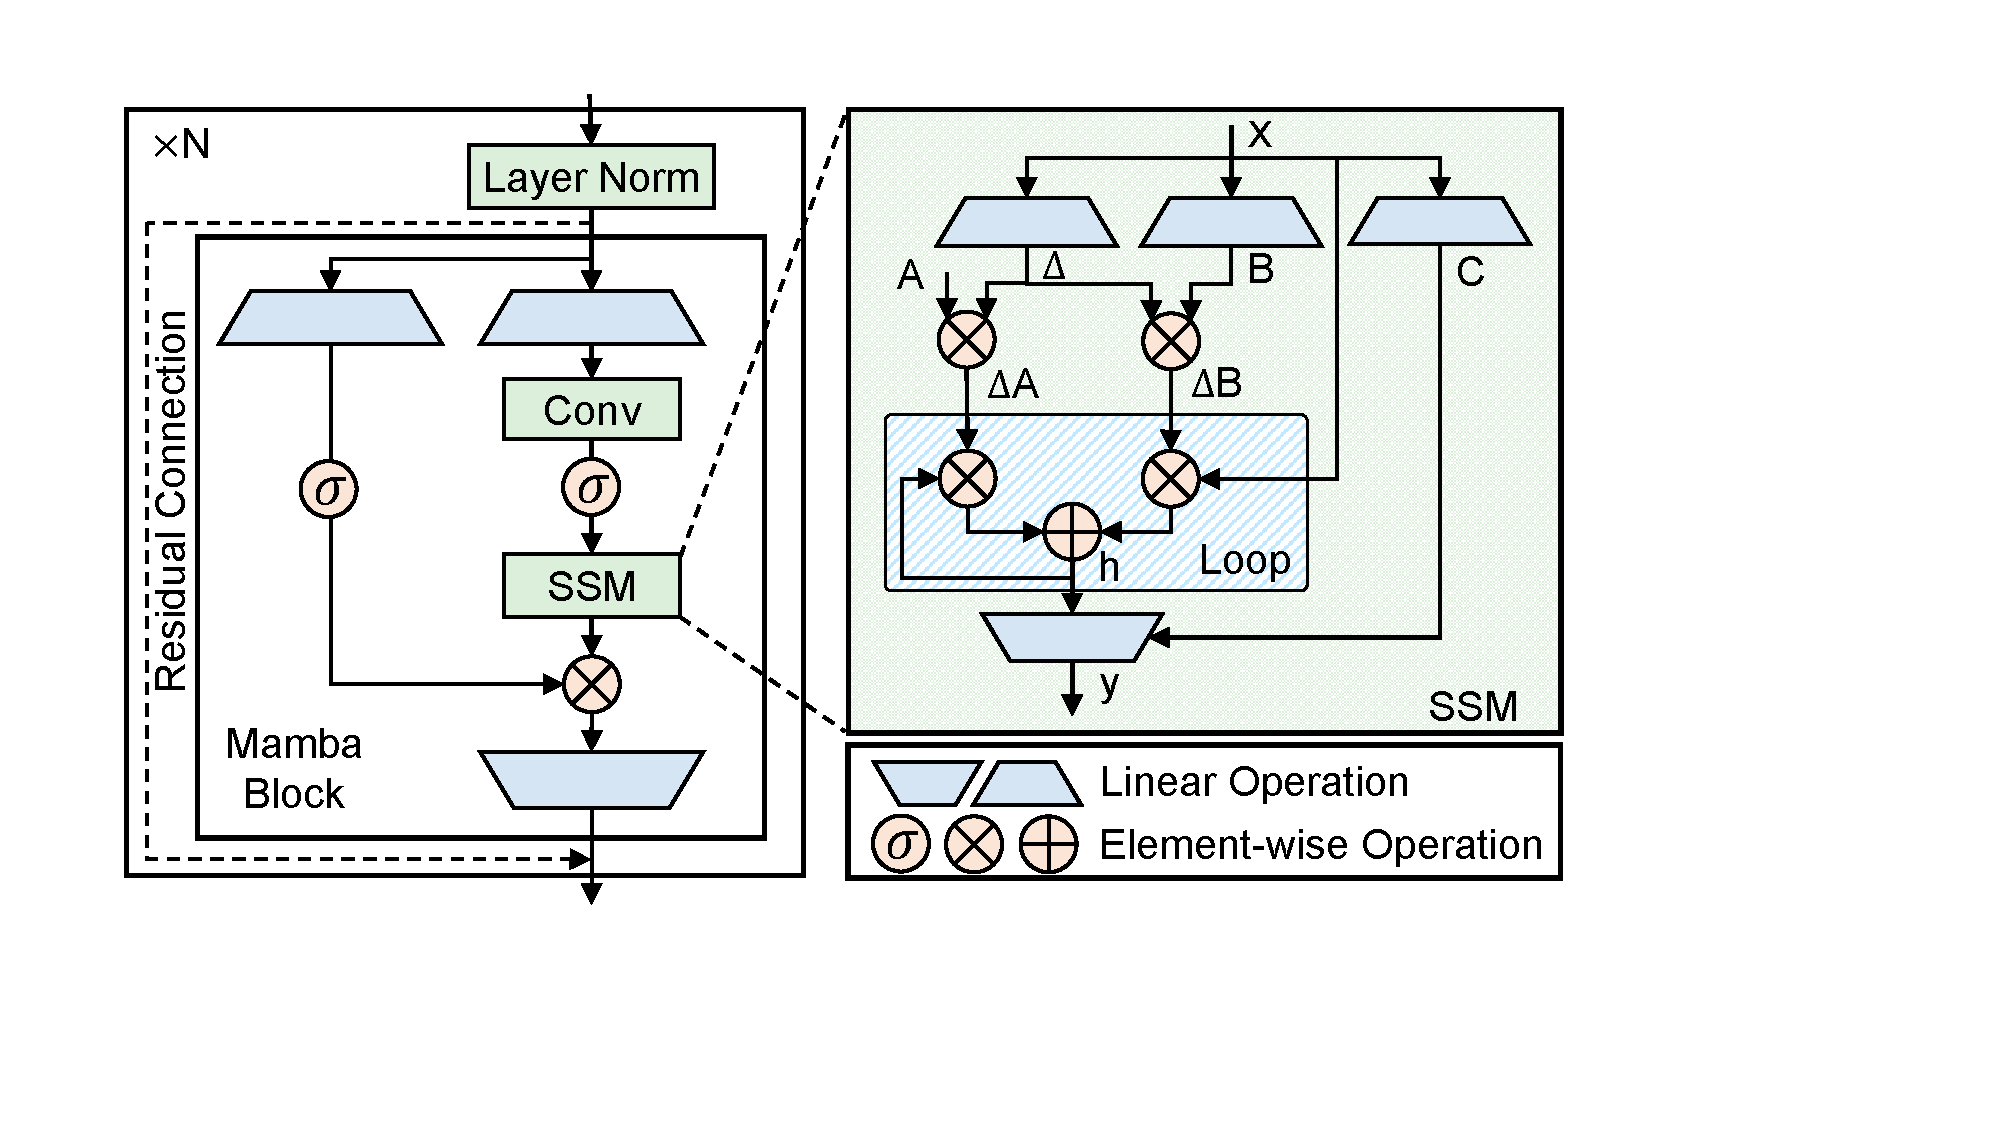
\includegraphics[width=0.47\textwidth]{figures/background/mamba_block.pdf}
%   \vspace{-16pt}
%   \caption{Computational flow in Mamba block and SSM. Mamba model consists of N blocks with residual connection. In SSM, $\Delta$, $B$ and $C$ are generated by input $x$. Then it performs loops to update hidden state $h$, and generates output $y$.}
%   \vspace{-18pt}
%   \label{fig:mamba_block}
% \end{figure}

% \subsection{Mamba}\label{sec:background:mamba}

% Mamba~\cite{mamba} introduces selective mechanism into SSM and proposes an implementation of selective state space model layer.
% Mamba block consists of a layer normalization, several linear projections, a convolution, a SSM block, and a residual connection.
% In each layer, the input sequence is first processed by a linear projection and then processed by the convolution.
% Then it is processed by an activation and then processed by the SSM. 
% After SSM, the main branch is multiplied by the collateral branch including a linear projection and an activation (\textit{e.g.}, SiLU~\cite{silu}) to generate the combined result.
% After combination, the result is processed by a linear projection.
% Last, the result is added back to the input through the residual connection~\cite{resnet}. 
% Instead of interleaving Mamba block and Feed-forward block, Mamba simply repeats the Mamba block homogenously. 

% During SSM processing, the input $x$ undergoes a series of transformations. 
% Firstly, it is subjected to three linear projections, resulting in $\Delta$, $B$ and $C$. 
% Subsequently, $\Delta$ is involved in the Einstein summation operations~\cite{einsum} with $A$ and $B$ separately, generating $\Delta A$ and $\Delta B$. 
% These intermediate results $\Delta A$ and $\Delta B$ are then multiplied with the hidden state and input $x$ by element-wise Einstein summation, respectively. 
% After $L$ (sequence length) times iterations, the hidden state is updated for $L$ times. 
% The outcomes of these operations are then combined through addition, resulting in the updated hidden state. 
% Finally, the updated hidden state undergoes matrix multiplication with $C$, followed by a linear transformation, to generate the output. The whole computational flow in Mamba block is illustrated in Figure \ref{fig:mamba_block}.



% \subsection{Tensor Core}\label{sec:background:tc}


\subsection{Memory Access Bottleneck}
The core of routing algorithms lies in the highly efficient heuristic path-planning method, like the A-star (or A$\ast$ ) search algorithm.  
However, the existing optimizations on the A* algorithm are mainly aimed at computational optimization, and the bottleneck in 
maintaining the open list and a closed list is obviously outstanding, especially when performing many iterative operations.  
For the typical path planning method (A*)acceleration by using FPGA, Zhou et al.[7] demonstrated 37-751$\times$ acceleration via 8-port cache 
and array-based OPEN lists, but the architecture suffers from inefficient resource utilization when processing high-obstacle density maps,
where frequent cache misses degrade performance predictability. 

Osama et al.[8] developed an FPGA implementation with 50-1001$\times$ speedup through 8-way parallel evaluators and cache-optimized memory access. 
Nevertheless, its fixed 256$\times$256 grid mapping and complex 5$\times$5 caching mechanism restrict scalability for large-scale scenarios. 
Jiang et al.[9] implemented an FPGA-based batched maze routing kernel achieving 3.11$\times$ speedup over CPU implementations with < 1\% 
wirelength degradation, but its performance is constrained by data dependency management and limited scalability when handling heterogeneous net sizes. 
Meanwhile, Lin et al.[10] proposed GAMER, a GPU-accelerated maze routing scheme that achieved 161$\times$ acceleration for coarsened maze routing through sweeping-style parallelism. 
However, its performance gain diminishes in fine-grained routing stages, and the qualitydriven batch partitioning strategy introduces 
additional scheduling overhead that limits throughput. 

\begin{figure}[htbp]
    \centering
    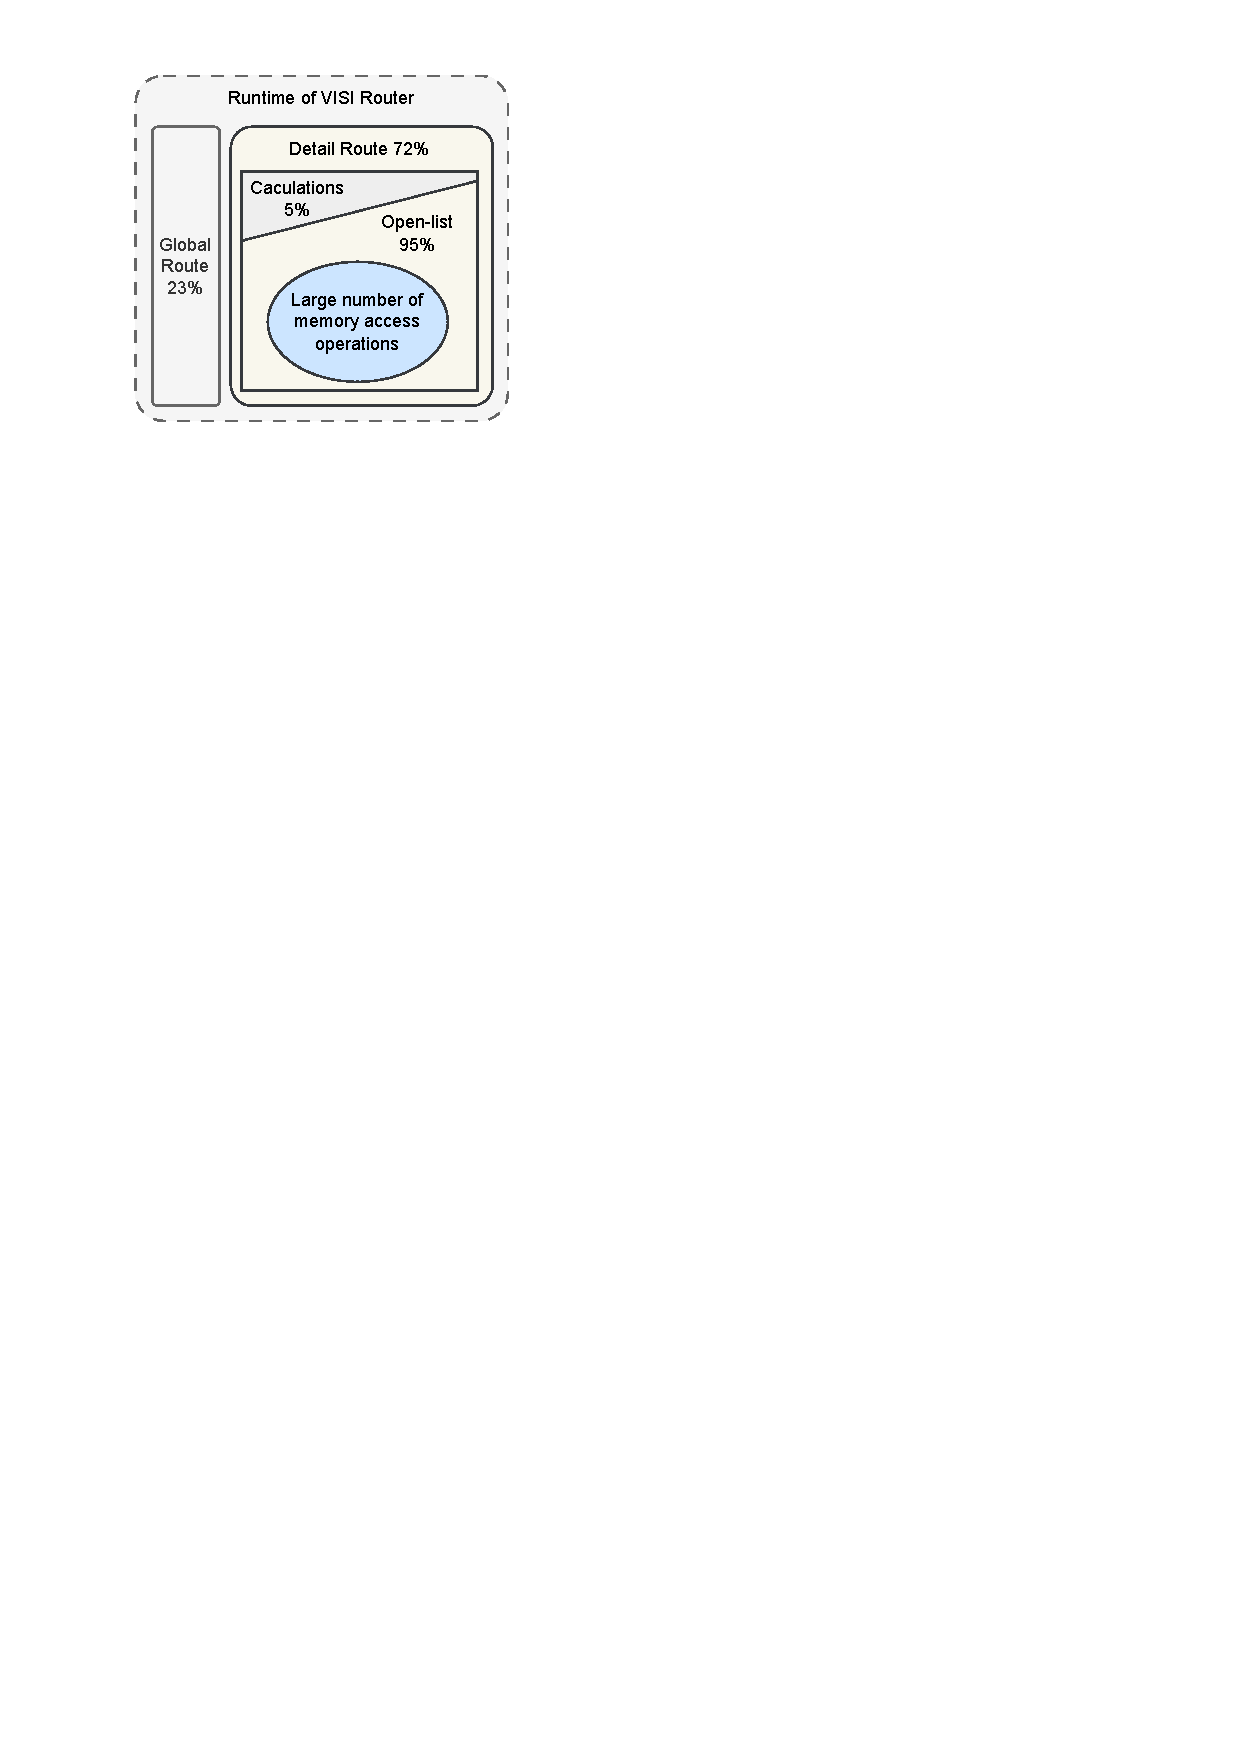
\includegraphics[width=7cm]{figures/background/Execution Time.pdf}
    \caption{Detailed routing takes up most time in the routing process, and most of it is memory access time.}
    \label{fig:Execution Time} % 标签紧跟标题
\end{figure}

\subsection{Versatility and Scalability}
The above proposed acceleration methodology for detailed routing preserves the quality of the entire implementation flow for 
multithreaded FPGA core architectures. Actually, the accelerated A* techniques exhibit broad applicability across various path-searching 
implementations. Given the fundamental similarities in routing paradigms,  particularly in maze routing algorithms and heuristic flow implementation 
methodologies, these acceleration strategies demonstrate significant transfer potential beyond the specific use cases examined in this study. 